\chapter{The First Law for Cosmological Solutions}
\label{ch:triplewick}

The planar solutions of the STU model came from considering the Nernst branes of \cite{Dempster:2015}, which were initially motivated by the search for black hole solutions obeying the strict third law of thermodynamics. We found that the Nernst-like behaviour of the solutions was lost as we increased the number of charges supported by the brane solution, but instead we gained a new class of cosmological solutions, where the external region of the spacetime is time-dependent and asymptotic to the Kasner solution. 

From the position of already thinking of black hole thermodynamics, it is then natural to the ask what thermodynamic properties these cosmological, planar horizons have. From our classification of trapping horizons in Section \ref{sec:stukruskalclassification}, it is possible to compute the temperature of the solution, and we can write down area densities which have an analogy in entropy density. Similarly, we can calculate the conserved charge densities $\mathcal{Q}$ and $\mathcal{P}$ associated to the solutions, together with chemical potentials, however, writing down a meaningful mass parameter has so far escaped us. In Section \ref{sec:emconservedcharges}, and Section \ref{sec:stumass}, we were able to write down a local expression for mass working in the finite, static region of spacetime, but as we were unable to set an overall normalisation, we cannot verify the first law, which is a differential relationship.

In Section \ref{sec:eucldeanactionformalism}, we saw that by Wick-rotating the gravitational action, we were able to make a formal equivalence between the gravitational and thermal partition functions. Computing the thermodynamic potential from the thermal partition function allows for the derivation of several thermodynamic parameters through partial derivatives of the free energy, including the internal energy. 

The standard simple Wick-rotation discussed in Section \ref{sec:eucldeanactionformalism} can be applied for static spacetimes which upon continuation remain real, so that the Euclidean on-shell action can be interpreted as a thermal partition function. The static patches of the planar solutions of Einstein-Maxwell model (Section \ref{sec:emsolutions}) and the STU model (Section \ref{sec:cosmologicalsolutionstu}) take the form
\begin{equation}
\label{static_patch}
ds^2 = - f(r) dt^2 + \frac{dr^2}{f(r)} + g(r)^2 (dx^2 + dy^2),
\end{equation}
which at first appears suitable for this procedure. However, we also need smooth field configurations to obtain a well-defined and finite Euclidean on-shell action. For the solutions we consider,  the static patches have a curvature singularity for some finite value $r=r_{\text{sing}}$ of the transverse coordinate $r$. We see that although we can Wick-rotate the line element and obtain a real, positive-definite spacetime, there will necessarily be a singularity within the Euclidean section and hence the Euclidean on-shell action is ill-defined. However, as we have seen, these static patches have a horizon at another finite value $r=r_h>r_{\text{sing}}$, and by analytic continuation we reach the external patch of the spacetime, which depends only on the coordinate $r$, which is timelike for $r  >r_h$. After relabelling $r \leftrightarrow t$, we can write the line element of these solutions into the form
\begin{equation}
\label{dynamic_patch}
ds^2 = - \frac{dt^2}{\tilde{f}(t)} + \tilde{f}(t) dr^2 + g(t)^2 (dx^2 + dy^2).
\end{equation}
Note that the function $\tilde{f}(t)$ has been modified with an additional sign: $\tilde{f}(x) = -f(x)$. This ensures that $\tilde{f}(t)$ is positive-definite within the domain of $t \in (t_h, \infty)$. For the remainder of the discussion, the tilde will be dropped and it is understood that functions $f$ appearing in the line element are positive-definite for each patch, and that the coordinate denoted $t$ is timelike while the coordinate denoted $r$ is spacelike.

These dynamic patches, where $t \in (t_h, \infty)$, more closely resemble the external, static patches of the Reissner-Nordst\"om solution we considered in our example in Section \ref{sec:rncausal}. However, in the dynamic patch, the horizontal Killing vector field is spacelike rather than timelike, and the application of the simple Wick-rotation leads to a complex line element and action. To work with this dynamic patch and ensure a real Euclidean section after Wick-rotation, we modify the standard Euclidean method. Before continuing, we note that there are some examples where complex line elements are used in the literature, the canonical example being the Kerr metric \cite{Gibbons:1976ue}. In this case, the generalisation is to admit timelike Killing vector fields which are not hypersurface orthogonal, and the complexification arises from cross terms in the line element. This is different from our case, where the Killing vector field is still hypersurface orthogonal, but spacelike. 

This chapter presents work initially completed in \cite{Gutowski:2020fzb}, which introduced a modification of the Euclidean action formalism though performing a \emph{triple Wick-rotation}. This method in principle can be applied to any metric which has no timelike-spacelike cross-terms, and depends explicitly on time but not on the spatial coordinates. Instead of Wick-rotating the time coordinate, we choose to Wick-rotate all three spacelike coordinates of the line element. As we are working exclusively with line elements of the form (\ref{dynamic_patch}), we denote the spatial coordinates $(r,x,y)$ such that the triple Wick-rotation takes the form
\begin{equation}
\label{eq:triplewick}
    (r,x,y) \rightarrow \pm i (r,x,y) ,
\end{equation}
where we admit either choice of sign. Notice that unlike the standard Wick-rotation, the resulting Euclidean line element will be \emph{negative-definite}, as we work with the mostly-plus conventions. As we saw in Section \ref{sec:eucldeanactionformalism}, the standard argument for identifying the resulting Euclidean action with a thermodynamic potential depends on the Killing vector being timelike, and thus being related to time translations and energy. In the dynamic outer patch, the Killing vector is spacelike and thus corresponds to spatial translations and momentum. This discrepancy from the standard formalism requires further work to understand fully, but we proceed formally and relate our Euclidean action to a thermodynamic potential, leaving questions about the underlying microscopic theory aside. The `energy' $E$ is defined as a derivative of this potential, and we prove that its variation $\delta E$ satisfies a relation which takes the exact form of the first law. As a further consistency check in Section \ref{sec:Isolated_horionzs}, we also apply the isolated horizon formalism, which imposes the first law and this way obtains an expression for the energy, and we find that the results of both formalisms agree.

In this chapter, we first discuss a general gravitational action, following the example of the single Wick-rotation in Section \ref{sec:eucldeanactionformalism}. From this, we write down a general expression for the Euclidean action after the triple Wick-rotation, which is then used in a series of examples. We begin considering the de Sitter solution in Section \ref{sec:desitter}. The de Sitter solution, when written in static coordinates, has an observer dependent cosmological horizon, but no singularity. This allows us to study the first law using the Euclidean action formalism for both the standard case in the finite-sized static region, and the triple Wick-rotation for the external dynamic region. Hence, the de Sitter solution is a perfect test case, used as a consistency check for the triple Wick-rotation. Following this, the planar solutions of the Einstein-Maxwell model (Section \ref{sec:thermopem}) and the STU model (Section \ref{sec:thermostu}) are analysed using the modified Euclidean action formalism, and we show that for both of these systems, the first law holds.

\section{Triple Wick-rotation}
\label{sec:triplewickrotation}

Following Section \ref{sec:eucldeanactionformalism}, the transformation \eq{triplewick} is applied to the gravitational action \eq{totact1} and the Euclidean action associated with the triple Wick-rotation is calculated. As with the standard Wick-rotation, we calculate the action term-by-term. The bulk contribution transforms as
\begin{equation*}
\begin{aligned}
    - \frac{1}{16\pi} \int_{M} (R - 2\Lambda) \sqrt{-g} d^4 x 
    \rightarrow 
     &- (\pm i)^{3}  \frac{1}{16\pi}  \int_{M} (R - 2\Lambda) \sqrt{-g} d^4 x ,\\
     = &\pm i \frac{1}{16\pi}  \int_{M} (R - 2\Lambda) \sqrt{-g} d^4x \;.
\end{aligned}
\end{equation*}
The GHY-term, as with the single Wick-rotation, transforms with the same sign for $\epsilon = \pm 1$.
\begin{enumerate}
    \item  
    For surfaces with a timelike unit normal
    \begin{equation*}
    	\epsilon = -1,  \qquad K \rightarrow K, \qquad \sqrt{\gamma} d^3x \rightarrow (\pm i)^{3} \sqrt{\gamma} d^3x.
    \end{equation*}
\item 
For surfaces with a spacelike unit normal, 
\begin{equation*}
	\epsilon = 1, \qquad K \rightarrow \mp i K, \qquad \sqrt{\gamma} d^3x \rightarrow (\pm i)^2 \sqrt{\gamma} d^3x,
\end{equation*}
\end{enumerate}
and we see that for either type of hypersurface, the GHY term transforms under a triple Wick-rotation as
\begin{equation*}
    + \frac{\epsilon}{8 \pi} \int_{\partial M} \sqrt{|\gamma|} (K - K_0) d^3x \rightarrow  \pm i \frac{1}{8 \pi} \int_{\partial M} \sqrt{|\gamma|} (K - K_0) d^3x.
\end{equation*}
Again, as with the standard Wick-rotation, we can write the gauge field contribution as a boundary term as we evaluate the action on shell. Performing the triple Wick-rotation, we find
\begin{equation*}
     \frac{1}{8 \pi} \int_{\partial M} F^{\mu \nu} A_{\mu} d\Sigma_{\nu} \rightarrow  \mp i \frac{1}{8 \pi} \int_{\partial M} F^{\mu \nu} A_{\mu} d\Sigma_{\nu},
\end{equation*}
where we have used that $d\Sigma_\mu \rightarrow (\pm i)^3 d\Sigma_\mu$, $A_\mu \rightarrow \pm iA_\mu$ and $F_{\mu \nu} \rightarrow \mp iF_{\mu \nu}$. Piecing this all together, the triple Wick-rotated Euclidean action is given by
\begin{equation}
\label{eq:3EucAct}
\begin{aligned}
        S_E = &\pm \frac{1}{16 \pi} \int_{M} \sqrt{g} (R - 2\Lambda) d^4 x ,
        \\& \pm \frac{1}{8\pi} \int_{\partial M} \sqrt{|\gamma|}(K-K_0) d^3x 
        \mp \frac{1}{8\pi} \int_{\partial M} F^{\mu \nu } A_\mu d\Sigma_\nu.
\end{aligned}
\end{equation}
We then (formally) identify the thermodynamic potential as we do in the standard formulation, evaluating the partition function $\mathcal{Z}$ in a saddle point approximation to obtain
\begin{equation}
\label{eq:thermalguess}
    \log \mathcal{Z} = - S_E(\beta, \mu) = - \beta \Omega,
\end{equation} 
where the inverse temperature $\beta$ and chemical potential $\mu$ can be expressed in terms of parameters of the triple-Wick-rotated solution. 

\section{Thermodynamics of the de Sitter solution}
\label{sec:desitter}

As an introductory example of the implementation of the triple Wick-rotation in spacetimes with dynamic asymptotic regions, we study the de Sitter solution. This example is somewhat simpler than the planar symmetric solutions considered in this thesis, as it is a vacuum solution without a curvature singularity.  However, it allows us to demonstrate that the results we obtain using a triple Wick-rotation in the dynamic patch agree with those obtained previously using a single Wick-rotation in the static patch. 

\subsection{Static patch, single Wick-rotation}
The de Sitter spacetime line element in static coordinates is given by
\begin{equation}
\label{eq:desitterline}
    ds^2 = -\left(1 - \frac{r^2}{L^2} \right) dt^2 + \left(1 - \frac{r^2}{L^2} \right)^{-1} dr^2 + r^2 d\Omega^2_2,
\end{equation}
with the cosmological horizon located at $r_h = L$, where $L$ is the de Sitter radius and the domain of our variable is $r \in [0,r_h)$. At $r=r_h$, there is a Killing horizon for the Killing vector field
$k^\mu = \partial_t$, which becomes spacelike when we continue to $r>r_h$. Unlike the event horizon for black hole solutions, the cosmological horizon in the de Sitter solution is observer dependent, and is formed by the spacelike separation of events due to the expansion of the spacetime. 

Using the Euclidean action formalism, the thermodynamics of de Sitter space can be calculated within the static patch $0 \leq r<r_h$ using standard methods. The cosmological constant $\Lambda$ can be written generally as a function of the de Sitter radius
\begin{equation*}
    \Lambda = -\frac{(D-1)(D-2)}{2 L^2} = -\frac{3}{L^2},
\end{equation*}
where for reference, we first give the relation for general dimension $D$ before setting $D=4$ for the remainder of our work. Note the non-conventional sign for the cosmological constant. We have decided within this thesis to have the cosmological constant to be proportional to the Ricci scalar, and in our conventions, a manifold with constant positive curvature has $R < 0$. We expand on this in Appendix \ref{app:conventions}.

Under the Wick-rotation $t \rightarrow -i \tau$, the line element \eq{desitterline} maps to the positive-definite line element 
\begin{equation}
\label{eq:eucds}
    ds^2 = \left(1 - \frac{r^2}{L^2} \right) d\tau^2 + \left(1 - \frac{r^2}{L^2} \right)^{-1} dr^2 + r^2 d\Omega^2_2.
\end{equation}

\paragraph{Entropy \& temperature}

Using the Bekenstein-Hawking area law, the entropy is determined by
\begin{equation}
\label{eq:dsBH}
    S_{dS} = \frac{A}{4} = \pi^2 L.
\end{equation}
The temperature associated with the horizon is proportional to the Kodama-Hayward surface gravity (\ref{eq:THK}) , which is found to be $\kappa = -L^{-1}$. Defining our thermodynamic horizon in the usual way, we look for the horizon crossed by future-directed causal geodesics which move from the exterior to the interior of the solution. These are the regions III and IV in Figure \ref{de_Sitter}, where the global time orientation is chosen such that the Killing vector field is future-pointing in region III, that is, globally time flows `upwards' in the diagram. This choice of regions is natural as it has the same causal structure as the part of the extended Schwarzschild spacetime which describes a black hole (regions I and II in the left diagram of Figure \ref{fig:sub1}). 

The line element \eq{desitterline} is in the same form as the cosmological solutions \eq{kruskalgen} we consider in Section \ref{sec:kruskalgen} and so we see that the horizon separating regions III and IV is a \emph{future inner horizon}, which has a temperature proportional to its surface gravity, thus yielding the Hawking temperature
\begin{equation*}
    T_H = \frac{\kappa}{2 \pi} = - \frac{1}{2\pi L}.
\end{equation*}
We note here that the sign of the temperature is different from the assignments made in other references, including \cite{Gibbons:1977mu, spradlin2001les}, where the Hawking temperature is positive $T_H>0$. However, according to \cite{spradlin2001les}, when the temperature is positive, it is found that entropy is negative. In our case, the sign of the temperature is determined by the type of trapping horizon, but the entropy is always defined by the area law and therefore positive. Note that the expression $TdS$ entering into the first law would be invariant for both approaches. 

\begin{figure}[!h]
\centering
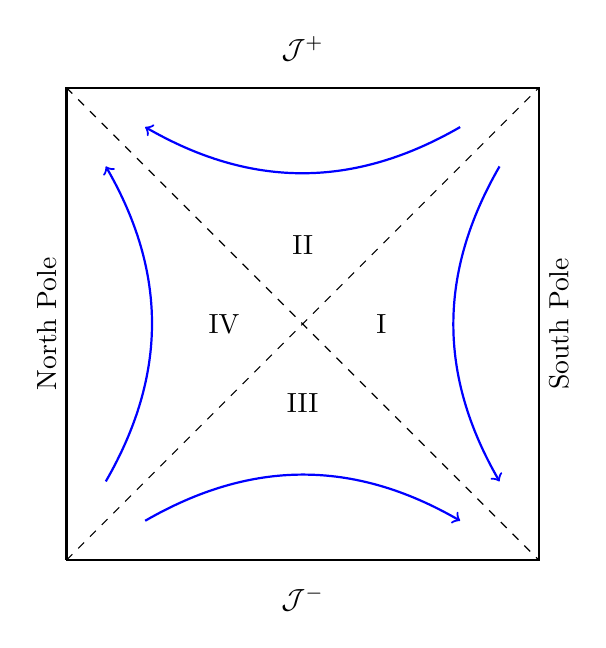
\begin{tikzpicture}
 	\draw[thick] (0,0) -- (6,0) node[midway,below=0.2cm] {$\mathcal{J}^-$}
   -- (6,6) node[rotate=90,midway,below] {South Pole}
   -- (0,6) node[midway,above=0.2cm] {$\mathcal{J}^+$}
   -- (0,0) node[rotate=90,midway,above] {North Pole};

	\draw[dashed] (0,0) -- (6,6);
	\draw[dashed] (0,6) -- (6,0);
	
	\draw[thick, blue, ->] (5.5,5) to [bend right] (5.5,1);
	\draw[thick, blue, ->] (0.5,1) to [bend right] (0.5,5);
	\draw[thick, blue, ->] (1,0.5) to [bend left] (5,0.5);
	\draw[thick, blue, ->] (5,5.5) to [bend left] (1,5.5);
	
	\node (a) at (4,3) {I};
	\node (a) at (2,3) {IV};
	\node (a) at (3,4) {II};
	\node (a) at (3,2) {III};
\end{tikzpicture}
\caption[Penrose-Carter diagram for the global de Sitter solution]{Penrose-Carter diagram for the global de Sitter solution. Dashed lines denote the cosmological horizon located for $r = L$ and the North/South poles are identified for $r = 0$. Blue curved arrows denote the flow of the Killing vector field. \label{de_Sitter}}
\end{figure}

\paragraph{Euclidean action}
Global de Sitter space is a maximally symmetric space of constant positive curvature with topology $\mathbb{R} \times S^3$. Its Kruskal diagram decomposes into four regions, two of which have a timelike Killing vector field and do not intersect the boundary, which is spacelike with topology $S^3$. If we evaluate the Euclidean action on a static patch, the boundary terms do not contribute and the de Sitter action is completely determined by the bulk terms: 
\begin{equation*}
    S_E = \frac{1}{16\pi} \int_{M} \sqrt{g}(R - 2\Lambda),
\end{equation*}
where the Ricci curvature is constant: $R = -12 L^{-2}$ and the integral over the four-manifold gives
\begin{equation*}
    S_E = \frac{1}{16\pi} \left(-\frac{6}{L^2}\right) \int_0^\beta d\tau \int_{S^2} \sin\theta d\theta d\phi \int_{r_h}^0 r^2 dr = -\pi L^2.
\end{equation*}
Note the limits on the integration of the radial coordinate $r$, which have been chosen to run from $r_h$, the origin of the Euclidean manifold, to the North pole for $r = 0$.\footnote{As this might be confusing, let us justify the integration bounds. Although we interpret $r = 0$ as the coordinate origin for static coordinates of the de Sitter solution, this is not the origin for the Wick-rotated Euclidean manifold. When we Wick-rotate, the location of the horizon: $r = r_h$, becomes the origin with the identification $\tau \simeq \tau + \beta$ made to avoid a conical singularity. Our integration limits are then chosen to match the conventions from the origin of the Euclidean space to the boundary and as such we integrate from $r = r_h$ to $r = 0$.} As there are no charges in the solution, we work in the canonical ensemble and we have the following relations:
\begin{equation*}
    \log(Z) = -S_E = -\beta F, \qquad F = E - T S .
\end{equation*}
The de Sitter solution is a maximally symmetric vacuum solution and thus interpreted as a ground state.  We therefore choose the natural normalisation $E=0$. Following from this we obtain
\begin{equation*}
    S_E = \beta F = - S \qquad \Rightarrow \qquad S = \pi L^2.
\end{equation*}
We see that the thermodynamic entropy matches with \eq{dsBH} and the first law is satisfied though in a `degenerate way', as the entropy is constant: $dS = 0 = TdS = dE = d(0) = 0$. 

We note that the negativity of the temperature: $\beta < 0$ for this example effects the boundedness of the partition function as the Euclidean action is negative: $S_E < 0$. If instead we had picked a positive temperature, we would return to the case considered within \cite{Gibbons:1977mu}, where $S_E > 0$, but the entropy of the solution has a sign difference from the Bekenstein-Hawking area law. We comment on this again in our discussion in Section \ref{sec:thermodiscussion}. 

\subsection{Dynamic patch, triple Wick-rotation}

The static patch is not complete and by analytical extension of the coordinate $r$ through the Killing horizon to values $r > r_h$, we obtain a second, dynamical patch, with asymptotic region $r \rightarrow \infty$. When crossing the horizon, the function $f(r)$ becomes negative, and we find that the coordinates $(t,r)$ exchange their roles. The timelike coordinate $t$ becomes spacelike, while the spacelike coordinate $r$ becomes timelike. We adopt the convention to relabel coordinates in the dynamic patch so that $t$ is always timelike and $r$ always spacelike. 

Then the line element in the dynamic patch is
\begin{equation}
\label{eq:desitterasy}
    ds^2 = -\left( \frac{t^2}{L^2} -1\right)^{-1} dt^2 +\left(\frac{t^2}{L^2} - 1\right) dr^2 + t^2 d\Omega^2_2\;.
\end{equation}
The coordinate domain is $t\in (t_h, \infty)$ where $t_h$ is the Killing horizon located at $t_h=L$. Note that while this cannot be read off from the local form of the line element, we have chosen the continuation from region IV to region III, so that $t \rightarrow \infty$ corresponds to past timelike infinity. This is relevant as it determines the sign of the temperature. 

\paragraph{Triple Wick-rotation}
We now perform a triple Wick-rotation where $r \rightarrow \pm i r$ and where the sphere $S^2$ is analytically continued to the hyperbolic plane $\Ham_2$ by $(\theta, \phi) \rightarrow \pm i (\theta, \phi)$. The line element \eq{desitterasy} is mapped to the \emph{negative-definite} line element
\begin{equation*}
    ds^2 = -\left( \frac{t^2}{L^2} -1\right)^{-1} dt^2 -\left(\frac{t^2}{L^2} - 1\right) dr^2 - t^2 d\Ham^2_2\;,\;\;\;
    d\Ham^2_2 = d\theta^2 + \sinh^2 \theta d\phi^2 \;.
\end{equation*}

\paragraph{Temperature \& entropy} The temperature and entropy associated with the Killing horizon are the same as in the previous calculation. Using the Kodama-Hayward expression \eq{THK}, the surface gravity is found to be $\kappa = -L^{-1}$ and for the future inner horizon between regions III and IV, the Hawking temperature is
\begin{equation*}
T_H = \frac{\kappa}{2\pi} =  - \frac{1}{2\pi L}.    
\end{equation*}
The entropy is identical to the static solution and is given by
\begin{equation*}
    S_{dS} = \frac{A}{4} = \pi^2 L.
\end{equation*}

\paragraph{Euclidean action}
The dynamical patches of global de Sitter space intersect the boundary, which is spacelike with topology $S^3$, therefore, we need to take boundary terms into account. After our triple Wick-rotation, the boundary has topology ${S}^1 \times \Ham_2$, where the radius of the $S^1$ is fixed by imposing the absence of a conical singularity. 

The Euclidean action for the triple-Wick-rotated system is 
\begin{equation*}
    S_E = \pm \frac{1}{16 \pi} \int_M \sqrt{g} (R-2\Lambda) d^4 x \pm \frac{1}{8 \pi} \int_{\partial M} \sqrt{\gamma} K d^3x  +  \int_{\partial M}  L_{ct}[\gamma] d^3x, 
\end{equation*}
where a counter term $L_{ct}$ has been included, which we will use to  remove divergences from the action. This method is the same as when calculating the Euclidean action for the more commonly considered asymptotically anti-de Sitter spacetimes \cite{Emparan_1999, Skenderis_2002}. We will take our boundary to be at $t \rightarrow \infty$, but to properly calculate the counter terms, we first integrate $t$ in the domain $t \in [t_h, \epsilon^{-1})$ and then take the limit of $\epsilon \rightarrow 0$. The volume
\begin{equation*}
   \omega = \int_{\Ham_2} \sinh \theta d\theta \wedge d\phi ,
\end{equation*}
of the hyperbolic plane is divergent. While one option in this situation is to work with densities, we keep $\omega$ as a formal constant which corresponds to the parametric volume $\omega_{S^2} = 4 \pi$ of the two-sphere in the static patch.

The bulk term of the Euclidean action is 
\begin{equation*}
    S_{\text{Bulk}} = \pm \frac{1}{16 \pi} \int_M \sqrt{g} (R-2\Lambda) d^4 x \;,
\end{equation*}
where
\begin{equation*}
    R = -\frac{12}{L^2}, \qquad \Lambda = -\frac{3}{L^2}, \qquad \sqrt{g} = t^2 \sinh \theta.
\end{equation*}
Putting these into the action and integrating over the manifold we find:
\begin{equation*}
    \begin{aligned}
        S_{\text{Bulk}} &= \pm \frac{1}{16 \pi} \int_M \sqrt{g} (R-2\Lambda)  d^4 x ,\\
        &= \pm \frac{1}{16 \pi} \left( -\frac{6}{L^2} \right) \int_0^\beta dr \int_{\Ham_2} \sinh \theta d\theta d\phi \int_L^{\epsilon^{-1}} dt \; t^2,\\
        &= \mp \frac{\beta \omega}{16 \pi} \frac{2}{L^2} \left(\frac{1}{\epsilon^3} - L^3\right) \;.
    \end{aligned} 
\end{equation*}
The Gibbons-Hawking-York term 
\begin{equation*}
    S_{\text{GHY}} =  \pm \frac{1}{8 \pi} \int_{\partial M} \sqrt{-\gamma} K d^3x,
\end{equation*}
can be calculated in the following way: the normal vector to the boundary for constant $t$ is
\begin{equation*}
    n^\mu = \left(- \sqrt{f}, 0, 0, 0 \right) \quad \Rightarrow \quad n_\mu n^\mu = -1.
\end{equation*}
The trace $K$ of the extrinsic curvature, evaluated on a surface of constant $t = t_0$, can then be computed using \eqref{K_as_divergence}:
\begin{equation*}
    K = \nabla_\mu n^\mu = \frac{3t_0^2 - 2L^2}{t_0 L^2 \sqrt{f}}, \qquad \sqrt{- \gamma} = \sqrt{f(t_0)} t_0^2 \sinh \theta
     \;,
\end{equation*}
such that 
\begin{equation*}
    K \sqrt{-\gamma} = \frac{3 t_0^3}{L^2} - 2t_0 \; .
\end{equation*}
Combining these, we find that the boundary contribution at $t_0 = \epsilon^{-1}$ is:
\begin{equation*}
    \begin{aligned}
        S_{GHY} &=  \pm \frac{1}{8 \pi} \int_{\partial M} \sqrt{-\gamma} K d^3x ,\\
        &= \pm \frac{1}{8 \pi} \left(\frac{3}{L^2 \epsilon^3} - \frac{2}{\epsilon} \right) \int_0^\beta dr \int_{\Ham_2} \sinh \theta d\theta d\phi , \\
        &= \pm \frac{\beta \omega}{8 \pi} \left(- \frac{2}{\epsilon} + \frac{3}{L^2 \epsilon^3}\right)  \;.
    \end{aligned}
\end{equation*}
The counter term is constructed from the geometric data of the boundary metric:
\begin{equation*}
    \int_{\partial M}  L_{ct}[\gamma] d^3x  = \int_{\partial M}  d^3x \sqrt{|\gamma|} (c_1 + c_2 R[\gamma]),
\end{equation*}
where $R[\gamma]$ is the Ricci curvature associated to the boundary manifold, and $c_{1,2}$ are renormalisation constants. We can expand out the counter terms in orders of $\epsilon$ and find:
\begin{equation*}
    \sqrt{|\gamma|} = \left(\frac{1}{L \epsilon^3} - \frac{L}{2 \epsilon} + \Op(\epsilon^1)  \right) \sinh \theta,
\end{equation*}
\begin{equation*}
    R[\gamma] \sqrt{|\gamma|} = \left(- \frac{2}{L \epsilon}  + \Op(\epsilon^1)  \right)\sinh \theta.
\end{equation*}
Comparing terms of order $\epsilon$ we find that the counter term is:
\begin{equation*}
    \int_{\partial M}  L_{ct}[\gamma] d^3x  = \mp \frac{1}{4 \pi L} \int_{\partial M} d^3x \sqrt{|\gamma|} \left(1 +  \frac{L^2}{4} R[\gamma] \right).
\end{equation*}
By construction, our action is now finite at the boundary $\epsilon \rightarrow 0$ and is of the form:
\begin{equation*}
    S_E = \pm \frac{\beta \omega}{8 \pi} \left(\frac{t_h^3}{L^2} \right) = \mp \frac{2 \pi L \omega}{8 \pi} \frac{L^3}{L^2} = \mp \frac{\omega L^2}{4}.
\end{equation*}
Picking the sign
\begin{equation*}
    (r,\theta,\phi) \rightarrow + i (r,\theta,\phi), 
\end{equation*}
for the triple Wick-rotation, the signs of the Euclidean actions agree for both patches, and the actions only differ by the numerical factors $\omega, \omega_{S^2}=4\pi $. As these are numbers, which we could eliminate by taking the Euclidean action per coordinate area, the resulting thermodynamics is the same. From the perspective of boundedness, we can pick our triple Wick-rotation such that $S_E > 0$. We will see in the following computations, the first law is recovered regardless of the sign of $S_E$. Furthermore, we find that the partition function is bounded from below naturally while satisfying other conditions. With this result, we continue to study the first law of thermodynamics for the solutions found in Chapters \ref{ch:planarem} and Chapters \ref{ch:planarstu}.

\section{Planar solutions of Einstein-Maxwell theory}
\label{sec:thermopem}

Our next example is the application of the triple Wick-rotation to the planar symmetric solutions of the Einstein-Maxwell equations, studied in Chapter \ref{ch:planarem}. We have seen in Section \ref{sec:emfromstu} that these solutions are the simplest examples of a class of planar solutions of the STU model, corresponding to the limit where all scalar fields are taken to be constant. We use these solutions as a starting point to study the thermodynamics of the planar symmetric solutions of STU model, as they already show all the qualitative features of the global causal structure of the full class of solutions. We will see from our computations that in this section, that the thermodynamics of planar Einstein-Maxwell solution is simpler than, but representative of, the thermodynamics of planar solutions of the STU model. 

Our starting point is the Lorentzian bulk action for Einstein-Maxwell theory \eq{EMaction}, repeated here for convenience 
\begin{equation*}    
        S  = \frac{1}{16\pi} \int d^4x \, \sqrt{-g} \,  \left( - R - F^2\right) .
\end{equation*}
In Section \ref{sec:emsolutions}, we found that solving the Einstein-Maxwell equations while imposing planar symmetry and staticity leads to a solution with the line element \eq{planareinsteinmaxwell}, repeated here
\begin{equation*}
    ds^2 = -f(r) dt^2 + \frac{dr^2}{f(r)} + r^2 (dx^2 + dy^2), \qquad f(r) = -\frac{2M}{r} + \frac{Q^2}{r^2},
\end{equation*}
where we remind the reader that the constant $M$ is taken to be positive to ensure the presence of a horizon. The transverse coordinate $r$ takes values in the interval $0 < r < r_h$, where $r=0$ is the location of a curvature singularity, while $r_h$ is the location of a  Killing horizon, where  $f(r_h) = 0$. 

We will assume that the solution only carries electric charge, the gauge field is given by
\begin{equation}
\label{eq:gaugefield}
    F = \left( - \frac{Q}{r} \right) dt \wedge dr\;.
\end{equation}
The gauge potential $A$ is found through integration of \eq{gaugefield} together with the standard boundary condition $A(r_h) = 0$:
\begin{equation}
\label{eq:gaugepotential}
    A = \left(- \frac{Q}{r} + \frac{Q}{r_h} \right) dt.
\end{equation}

\paragraph{Charge \& chemical potential}
The chemical potential is given by the asymptotic value of the gauge potential \cite{Hartnoll:2009sz}; taking this limit for \eq{gaugepotential} gives 
\begin{equation*}
    \mu :=  \lim_{r \rightarrow \infty} A_t = \frac{Q}{r_h} = \frac{2 M}{Q} \;.
\end{equation*}
Note that while $r \rightarrow \infty$ is outside the static patch $0<r<r_h$, we will see below that we can analytically extend spacetime to $0<r<\infty$, so that this limit makes sense. The conserved electric charge was computed using Gauss' law \eq{pemcharge}, which was found to be
\begin{equation*}
    \mathcal{Q} = \lim_{r \to \infty} \frac{1}{4\pi} \int_{\Real^2} \star F = \frac{Q \omega}{4\pi}, \qquad \omega = \int_{\Real^2} dx \wedge dy \;.
\end{equation*}
Here $\omega$ is the divergent parametric area of the horizon. The factor of $4\pi$ is due to the normalisation we have chosen for the gauge field. In our conventions the volume form is defined using the conventional choice $\epsilon_{trxy} = 1$.

\subsection{Dynamic patch}

Due to the presence of a curvature singularity at $r=0$ we cannot apply the standard thermodynamic formalism in the static patch. In Section \ref{sec:dynamicem} we analytically continued our coordinates using advanced Eddington-Finkelstein coordinates at an intermediate step to extend spacetime to the dynamical region $r_h < r < \infty$, where the horizontal Killing vector field became spacelike. As $r$ becomes a timelike coordinate in the dynamic patch, we apply the same convention as in the de Sitter example and relabel the coordinates $(t,r) \rightarrow (r,t)$, and redefine $f$ by a minus sign. Then the line element of the dynamic patch takes the form \eq{Region_II}, repeated here
\begin{equation}
\label{eq:planarEM2}
    ds^2 = -\frac{dt^{2}}{f(t)} +  f(t) dr^{ 2}  + t^{2} (dx^2 + dy^2) ,\qquad f(t) = \frac{2M}{t} - \frac{Q^2}{t^2} , \qquad t_h = \frac{Q^2}{2M}.
\end{equation}
This line element covers region III of Figure \ref{fig:PC}, with $t\rightarrow \infty$ corresponding to past timelike infinity. Using advanced Eddington-Finkelstein coordinates, one can show that the Killing horizon between regions III and IV (and I) is an apparent horizon of \emph{future inner type}, consistent with the interpretation as a contracting cosmological solution. We saw this in Section \ref{sec:pemglobal} from the point of view of Kruskal coordinates and the expansion of null congruences. We could alternatively classify the horizons of the solution using advanced/retarded Eddington-Finkelstein coordinates which are correlated with past/future timelike infinity. For further discussion on this, we refer to Appendix D in \cite{Gutowski:2020fzb}.

\paragraph{Temperature \& entropy}

To compute the surface gravity and temperature of the future inner horizon, we use the Kodama-Hayward formalism to compute the surface gravity. From Section \ref{sec:pemglobal}, we understand the regions III and IV to be separated by a future inner horizon and so $T_H \propto \kappa$. Applying \eq{THK} to the line element \eq{planarEM2}, we obtain
\begin{equation}
\label{eq:EMtemp}
    \kappa = - \frac{4M^3}{Q^4} \quad \Rightarrow \quad T_H = \frac{\kappa}{2\pi} = - \frac{2 M^3}{\pi Q^4}.
\end{equation}
The Bekenstein-Hawking area law gives a relation for the entropy of the horizon in terms of the horizon area: 
\begin{equation*}
    S_{BH} = \frac{A}{4} = \frac{\omega t_h^2}{4} = \frac{Q^4 \omega}{16M^2}.
\end{equation*}
As with other extensive quantities, we keep the divergent volume $\omega$ as a formal constant rather than using densities. 

\subsection{Euclidean action}

Our main goal is to show that the future inner horizon satisfies the first law of Killing horizon mechanics, which takes the same form as the first law of thermodynamics. This requires us to identify geometrically defined quantities of the solution with thermodynamic quantities. In standard black hole thermodynamics, the mass $M$ of the black hole is identified with the internal energy of a canonical or grand canonical ensemble. Due to the planar symmetry, and since we are not working in a static patch, we do not have a natural candidate for a mass-like quantity. We will trade this problem for the one of obtaining a well behaved Euclidean action which we interpret as a grand canonical partition function. The mass-like quantity we identify with the internal energy is then obtained using standard thermodynamic relations. The remaining problem in defining the Euclidean action is its normalisation. For solutions which are asymptotic to a `vacuum',  that is to a maximally symmetric spacetime, the normalisation is fixed by including a boundary term such that the Euclidean action is zero when evaluated on the vacuum solution. We do not have this option as our solution is not asymptotic to a maximally symmetric spacetime. Moreover, the GHY-boundary term will turn out to be finite, so there is no natural candidate for a boundary counter term. However, the integral over the two planar directions is divergent, and while we can formally absorb this in a constant $\omega$, we will allow for a finite multiplicative factor $\mathcal{N}$ between the Euclidean action $S_E$ and the grand potential $\Omega$:
\begin{equation}
\beta \Omega = \mathcal{N} S_E \;.
\end{equation}
The constant $\mathcal{N}$ parametrises the relative normalisation between thermodynamic and geometric quantities. To fix it, we impose one relation, which we choose to be Gauss' law. That is, we identify the charge $\mathcal{Q}$ defined by the gauge field of our field configuration with the negative derivative of $\Omega$ with respect to the chemical potential
\begin{equation}
\label{eq:EMBoundary}
    \pardev{\Omega}{\mu} \overset{!}{=} - \mathcal{Q} \;.
\end{equation} 
Once $\mathcal{N}$ has been fixed by this condition, all thermodynamic relations must take their standard form, if our interpretation of $\mathcal{Z} = \exp( -\mathcal{N} S_E)$ as a thermodynamic partition function is correct. 

Performing the triple Wick-rotation
\begin{equation*}
    (r,x,y) \rightarrow \pm i ({r}, {x},{y}),
\end{equation*}
we obtain the negative-definite line element
\begin{equation}
    ds^2 = -f(t)^{-1} dt^2 - f(t) d{r}^2 - t^2 (d{x}^2 + d{y}^2).
\end{equation}
The Euclidean action is given by
\begin{equation*}
\begin{aligned}
        S_E = &\pm \frac{1}{16 \pi} \int_{M} \sqrt{g} R d^4 x \pm \frac{1}{8\pi} \int_{\partial M} \sqrt{|\gamma|}Kd^3x , \\
        &\mp \frac{1}{8\pi} \int_{\partial M} F^{\mu \nu } A_\mu d\Sigma_\nu.
\end{aligned}
\end{equation*}
Since the planar Einstein-Maxwell solution has a vanishing Ricci scalar: $R = 0$, the action is completely determined by the boundary terms, which are evaluated in the limit where $t \rightarrow \infty$. We do not include a background boundary term $K_0$, as $S_E$ will turn out to be finite. 

The hypersurface $\Sigma = \partial M$ is obtained as the limit of a sequence of slices of the spacetime $M$ for constant time $t_0$, and has an extrinsic curvature with trace $K$ when considered as an embedded submanifold of $M$. It can be computed using the formulas reviewed in Section \ref{sec:extrinsic} and we obtain the result
\begin{equation*}
    K = \frac{3Mt_0 -Q^2}{t_0^2 \sqrt{2 M t_0 - Q^2}} ,\qquad \sqrt{|\gamma|} = t_0^2 \; \left( \frac{2M}{t_0} - \frac{Q^2}{t_0^2} \right)^{\half}.
\end{equation*}
Evaluating this in the limit $t_0 \rightarrow \infty$ gives
\begin{equation*}
    S_{GHY} = \pm \frac{1}{8\pi} \int_{\partial M} \sqrt{|\gamma|} K  = \pm 
    \frac{3 M \beta \omega}{8\pi} \;.
    \end{equation*}
The factor $\beta \omega$ is the parametric volume of the boundary.     
After Wick-rotation, the coordinate $r$ becomes periodic with period $\beta$, in order to avoid a conical singularity at $t=t_h$.\footnote{To be precise, the conical method determines the period up to sign, and we choose $\beta$ to have the sign determined by the Kodama-Hayward method.}     
    
As the gauge potential has only one non zero component, so the boundary term is calculated
\begin{equation*}
        \mp \frac{1}{8\pi} \int_{\partial M} F^{\mu \nu } A_\mu d\Sigma_\nu
    =  \pm \frac{M \beta \omega}{4 \pi}.
\end{equation*}
Together, the GHY-term and the gauge field contribution yield the Euclidean action
\begin{equation}
\label{eq:emeucact}
    S_E = \pm  5 \frac{M \beta  \omega}{8 \pi} \;.
\end{equation}

\subsection{Verifying the first law}

Formally equating the partition function calculated from the Euclidean action with the negative logarithm of the thermal partition function, $\log(\mathcal{Z}) = -\mathcal{N} S_E = -\beta \Omega$,  yields the grand potential
\begin{equation*}
    \Omega(\beta, \mu) = \frac{\mathcal{N} S_E}{\beta} = 
    \mp 5 \mathcal{N}  \frac{\beta  \mu ^4 \omega}{(8 \pi)^2} \;,
\end{equation*}
which we have written in terms of its natural thermodynamic
variables $\beta=T_H^{-1}$ and $\mu$ using the relationship
\begin{equation*}
    M = - \frac{\beta \mu^4}{8 \pi}, \qquad \mathcal{Q} = -\frac{\mu^3 \beta \omega}{(4\pi)^2}.
\end{equation*} 
We now apply our normalisation condition \eq{EMBoundary}: 
the conserved charge $\mathcal{Q}$ calculated from Gauss' law must match the negative $\mu$-derivative of $\Omega$. Taking the derivative, we find that
\begin{equation*}
	- \pardev{\Omega}{\mu} = \pm 5 \N \frac{4 \beta \mu^3 \omega}{ (8\pi)^2} = \pm 5 \N \mathcal{Q}, \quad \Rightarrow \quad \N = \mp \frac{1}{5}.
\end{equation*}
From this, the grand potential and partition function are determined to be
\begin{equation}
\label{eq:grandplanarem} 
\Omega(\beta, \mu) =  \frac{\beta  \mu ^4 \omega}{(8 \pi)^2}, \qquad \log(\mathcal{Z}) = - \frac{\beta^2 \mu^4 \omega}{(8\pi)^2}  \;.
\end{equation}
and we see that the partition function is bounded from below.

The free energy $F(\beta, \mathcal{Q})$ is obtained as the  Legendre transform of the grand potential
\begin{equation}
\label{eq:RNfreeenergy1}
    F(\beta,\mathcal{Q}) = \Omega -  \mu \frac{\partial \Omega}{\partial \mu} = 
    \Omega + \mu \mathcal{Q} = 
    3 \left(-\frac{\pi^2 \mathcal{Q}^4}{4 \beta \omega} \right)^{\frac{1}{3}}\;,
\end{equation} 
where we have used the relation 
\begin{equation*}
    \mu = \left(- \frac{16 \pi^2 \mathcal{Q}}{\omega \beta} \right)^{1/3} \;,
\end{equation*}
to express the free energy in terms of its natural variables $\beta$ and $\mathcal{Q}$. 
From $F$ we can compute the thermodynamic entropy $S$ and check that it matches the Bekenstein-Hawking entropy $S_{BH}:$ 
\begin{equation}
\label{eq:entEM}
    S = \beta^2 \pardev{F}{\beta} 
    = \left( \frac{\pi^2 \mathcal{Q}^4 \beta^2}{4 \omega} \right)^{\frac{1}{3}}
    = S_{BH}  \;.
\end{equation}
As a further consistency check, we can also verify that the free energy gives us the correct chemical potential:
\begin{equation*}
    \pardev{F}{\mathcal{Q}} = \left(- \frac{16 \pi^2 \mathcal{Q}}{\beta \omega} \right)^{1/3} =  \mu.
\end{equation*}
The internal energy $E$, for which we do not have a geometric definition, is computed from the free energy:
\begin{equation*}
E =    \pardev{(F \beta)}{\beta} = 
 \left(- \frac{2 \pi^2 \mathcal{Q}^4  }{\beta \omega} \right)^{1/3} = \frac{M\omega}{4\pi} \;.
\end{equation*}
We observe that $E$ is proportional to the parameter $M$, and therefore $E$ is positive. Notice that like the de Sitter solution, if we set the area density to $\omega = 4\pi$, we obtain $E = M$.  Looking back to \eq{pemkomar}, we see that the mass we compute here matches the naive asymptotic limit of the Komar energy. In both the triple Wick-rotation and in the Komar `mass', we could think of the mass-like parameter being associated to a momentum like quantity, and so it is interesting to see how they match.

Using our previous results we can verify that the thermodynamic variables $E,T,S,\mu, \mathcal{Q}$ satisfy the Smarr relation
\begin{equation}
E = 2TS + \mu \mathcal{Q}  \;.
\end{equation}
Expressing the internal energy $E$ in terms of its natural variables $S$ and $\mathcal{Q}$, we obtain the equation of state
\begin{equation*}
    E(S,\mathcal{Q}) = \frac{\pi \mathcal{Q}^2 }{(S \omega)^{1/2}} \;.
\end{equation*}
The partial derivates of the internal energy are 
\begin{equation*}
    \pardev{E}{S} = - \frac{\pi \mathcal{Q}^2}{2 S^{3/2} \omega^{1/2}} = \frac{1}{\beta} = T, \qquad     \pardev{E}{\mathcal{Q}} = \frac{2 \pi \mathcal{Q}}{(S \omega)^{1/2}} = \mu,
\end{equation*}
where both expressions have been simplified by substituting in $S(\beta, \mathcal{Q})$ using \eq{entEM}. The variation of the internal energy is
\begin{equation*}
    dE = \pardev{E}{S} dS + \pardev{E}{\mathcal{Q}} d\mathcal{Q}
       = T dS + \mu d\mathcal{Q} \;.
\end{equation*}
This relation takes the standard form of the first law of thermodynamics. Note that this works because we have allowed that the temperature is negative. If we had insisted that the temperature is positive, this would have resulted in a non-standard sign for the entropy term. 

\section{Planar solutions of the STU model}
\label{sec:thermostu}

We are now in a position to turn to our main application of the triple Wick-rotation; the planar cosmological solutions of the STU model found in Chapter \ref{ch:planarstu}, for which we will now verify the first law of thermodynamics. To aid our discussion, we repeat the bosonic Lagrangian for $n_V$ vector multiplets coupled to ${\cal N}=2$ supergravity
\begin{equation}
\label{Bos_Lag}
 e_4^{-1} \La = -\frac{1}{2 \kappa_4^2}R - \frac{1}{\kappa_4^2} g_{A\bar{B}} \partial_\mu z^A \partial^\mu \bar{z}^{\bar{B}} + \frac{1}{4 \kappa_4^2} \I_{IJ} F^I_{\mu \nu} F^{J|\mu \nu} + \frac{1}{4 \kappa_4^2} \cR_{IJ} F^I_{\mu \nu} \tilde{F}^{J|\mu \nu},
\end{equation}
where compared to \eq{4dlag}, we have restored the four-dimensional gravitational coupling $\kappa_4$ by an overall scaling to maintain the form of our solutions. While we used standard supergravity conventions where $\kappa_4^2 = 1$ in Chapter \ref{ch:planarstu}, it will be more convenient in the following to use relativist's conventions where $G=1$ and $\kappa_4^2 = 8\pi$, in order to avoid non-standard numerical factors in thermodynamic relations. We remind the reader that the couplings $g_{A\bar{B}}, \; \I_{IJ}$ and $\cR_{IJ}$, where $A,B = 1, \ldots, n$ and $I,J = 0, \ldots, n$ are functions of the scalar fields $z^A$ \eq{stuphysicalscalars}, and their exact form is derived in Appendix \ref{app:stucouplings}. 

\subsection{Dynamic patch}
\label{sec:studynamicthermo}
As in the solutions of Einstein-Maxwell, we begin with the line element in the dynamical patch of the planar symmetric cosmological solution 
\begin{equation}
\label{eq:STUline}
    ds^2  = - \frac{\Ham(\zeta)}{\cW(\zeta)} d\zeta^2 +  \frac{\cW(\zeta)}{\Ham(\zeta)} d\eta^2 +  G(\zeta)  (dx^2 + dy^2),
\end{equation}
where all functions depend only on the timelike coordinate $\zeta$:
\begin{equation*}
\begin{aligned}
    \cW(\zeta) &= \alpha \zeta - 1, \\
    \Ham_a(\zeta) &= (\beta_a + \gamma_a \zeta) ,\\
    \Ham(\zeta) &= 2 \left(\Ham_0 \Ham_1 \Ham_2 \Ham_3 \right)^{\half}, \\
    G(\zeta) &= \zeta^2  \left[\left(1 + \frac{\beta_0}{\gamma_0 \zeta}\right)\left(1 + \frac{\beta_1}{\gamma_1 \zeta}\right)\left(1 + \frac{\beta_2}{\gamma_2 \zeta}\right)\left(1 + \frac{\beta_3}{\gamma_3 \zeta}\right)\right]^{\half}.
\end{aligned}
\end{equation*}
This line element has been modified compared to \eq{4chargenew}, through the rescaling of the planar coordinates $(\bar{x},\bar{y}) \mapsto (x,y)$ such that the corresponding part of the line element is now
 \begin{equation*}
 \begin{aligned}
          \Ham(\zeta) (d\bar{x}^2 + d\bar{y}^2) &= 2\sqrt{\gamma_0\gamma_1\gamma_2\gamma_3} \; G(\zeta) (d\bar{x}^2 + d\bar{y}^2), \\ &=  G(\zeta)(dx^2 + dy^2)  \;.
 \end{aligned}
 \end{equation*}
 This rescaling has been chosen such that the asymptotic form of the planar line element is $ds^2_2 = \zeta^2(dx^2 + dy^2)$. In this form, the line element matches the planar Einstein-Maxwell solutions which asymptotically is given by $ds^2_2 = t^2 (dx^2 + dy^2)$. We note that as the line element has no functional dependence on the planar coordinates, we could rescale them by an arbitrary function of the thermodynamic data; the choice that we make here appears to be the most natural.
 
 In the following calculations we will rewrite expressions using the integration constants found in Section \ref{sec:cosmologicalsolutionstu}. We repeat here the relations between the integration constants found while solving the equations of motion in Section \ref{sec:stueucinstanton} and the ones appear in \eq{STUline}
\begin{equation}
\label{eq:stuintconst}
    \begin{aligned}
        \beta_a = \frac{2 K_a}{\alpha} \sinh \bigg(\frac{\alpha h_a}{2 K_a}\bigg), \qquad
        \gamma_a = K_a \exp \left(-\frac{\alpha h_a}{2 K_a} \right),
    \end{aligned}
\end{equation}
where 
\[
K_a = \left(Q_0, P^1, P^2, P^3 \right),
\]
are the four non-zero charges carried by the gauge fields $F^I_{\mu \nu}$.\footnote{We drop the sign in front of $Q_0$ within $K_a$ as it allows us to drop the various modulus signs in our integration constants.} Without loss of generality, we can take the set of integration constants $\{\alpha, K_a, h_a \}$ to be non-negative. We will work with the gauge fields \eq{new4dgauge}, which are given by
\begin{equation}
\label{eq:firstlawgaugefield}
    \begin{aligned}
        F^0_{\zeta \eta} =  -\frac{Q_0}{2(\beta_0 + \gamma_0 \zeta)^2}, \qquad \tilde{F}_{A |\zeta \eta} = \frac{P^A}{2(\beta_A + \gamma_A \zeta)^2}.
    \end{aligned}
\end{equation}
where we explicitly note that we choose to work with $\tilde{F}_{A|\mu \nu}$, which denote the duals of the gauge field $F^A_{\mu \nu}$. The advantage of using the fields $(F^0, \tilde{F}_A)$ instead of $(F^0, F^A)$ is that now all gauge fields and charges appearing in the solution are electric,\footnote{This is for computational simplicity. In \cite{Hawking:1995ap}, the authors show how magnetic and electric black hole solutions are equivalent in the semi-classical approach applied here.} allowing us to treat all contributions the same thermodynamically. Note that as the gauge couplings are field dependent, dualisation is not just Hodge-star, but additionally involves inverting the couplings. This was discussed in Section \ref{sec:electromagneticduality} for the general case of $\N = 2$ supergravity. The precise relation between gauge fields and dual gauge fields is
\begin{equation*}
    \tilde{F}_A = - \star \I_{AB} F^B \quad \Rightarrow \quad F^A = \star \I^{AB} \tilde{F}_B,
\end{equation*}
where $F^A, \tilde{F}_A$ are the two-forms corresponding to the gauge fields. Note that the coupling matrix $\I_{IJ}$ is invertible, and in our convention is negative-definite. 

\paragraph{Temperature}
In Section \ref{sec:stukruskalclassification}, we saw that the Killing horizon located at $\zeta = \zeta_h = \alpha^{-1}$ is a \emph{future inner horizon} and hence $T_H \propto \kappa$. The surface gravity is computed using the Kodama-Hayward formulation \eq{THK} and we find that the temperature is negative, and of the form
\begin{equation}
\label{eq:STUtemp}
\begin{aligned}
        T_H &= -\frac{1}{4 \pi} \partial_\zeta \left(\frac{\cW(\zeta)}{\Ham (\zeta)} \right) 
        \bigg|_{\zeta=\alpha^{-1}} , \\
        &= -\frac{\alpha^{3}}{8 \pi} \left[\left(\alpha  \beta _0+\gamma _0\right) \left(\alpha  \beta
   _1+\gamma _1\right) \left(\alpha  \beta _2+\gamma _2\right) \left(\alpha  \beta
   _3+\gamma _3\right) \right]^{-\half}.
\end{aligned}
\end{equation}
Using the relations above \eq{stuintconst},  we can simplify the expression of the temperature to 
\begin{equation*}
    (\alpha \beta_a + \gamma_a) = K_a \exp\left(\frac{\alpha h_a}{2 K_a} \right) = \frac{K_a^2}{\gamma_a} \quad \Rightarrow \quad    T_H = -\frac{\alpha^3}{8 \pi} \frac{\sqrt{\gamma_0 \gamma_1 \gamma_2 \gamma_3}}{Q_0 P^1 P^2 P^3}.
\end{equation*}

\paragraph{Entropy} Using the Bekenstein-Hawking area law we can compute the entropy density of the solution:
\begin{equation*}
\begin{aligned}
        S_{BH} &= \frac{G(\zeta_h)}{4} = \frac{1}{4 \alpha^2} \exp\left[\frac{\alpha}{2} \left(\frac{h_0}{Q_0} + \frac{h_1}{P^1} + \frac{h_2}{P^2}+\frac{h_3}{P^3} \right) \right],  \\
        &= \frac{1}{4 \alpha^2} \frac{Q_0 P^1  P^2 P^3}{\gamma_0 \gamma_1 \gamma_2 \gamma_3}.
\end{aligned}
\end{equation*}
Since the planar STU solution has several integration constants, we will suppress the parametric volume $\omega$ of the planar directions in this section by setting $\omega=1$. This can be interpreted as either working with densities of divergent extensive quantities, or as compactifying the planar dimensions on a two-torus with unit area. 

\paragraph{Chemical potentials}

The corresponding gauge potentials are found by integration of the gauge fields \eq{firstlawgaugefield}, subject to the standard boundary condition $A(\zeta_h) = \tilde{A}(\zeta_h) = 0$:
\begin{equation*}
    (A^{0})_\eta = -\frac{\gamma_0 (\alpha  \zeta -1)}{2 Q_0 \left(\beta _0+\gamma_0  \zeta \right)} ,
\qquad
    (\tilde{A}_{A})_\eta = \frac{\gamma_A (\alpha  \zeta -1)}{2 P^A \left(\beta_A+\gamma_A  \zeta \right)} .
\end{equation*}
We then take the asymptotic limit of the gauge potentials to obtain the chemical potentials
\begin{equation*}
    \mu^0 := \lim_{\zeta \rightarrow \infty} A^0_\eta = -\frac{\alpha}{2Q_0}, 
    \qquad 
    \tilde{\mu}_A := \lim_{\zeta \rightarrow \infty} \tilde{A}_{A |\eta} = \frac{\alpha}{2P^A}. 
\end{equation*}

\paragraph{Electromagnetic charges}

As with the Einstein-Maxwell solution, the conserved charges are computed using Gauss' law. However, we need to take into account that the gauge couplings depend on the scalar fields. The gauge field couplings come from $\I_{IJ}$ and were calculated explicitly in \eq{iij_coupling}
\begin{equation*}
    \I_{IJ} = \text{diag} \left(-stu, -\frac{tu}{s}, -\frac{su}{t}, -\frac{st}{u} \right),
\qquad
    \I^{IJ} = \text{diag} \left(-\frac{1}{stu}, -\frac{s}{tu}, -\frac{t}{su}, -\frac{u}{st} \right),
\end{equation*}
where
\begin{equation*}
    s = -\text{Im}(z^1), \qquad t = -\text{Im}(z^2), \qquad u = -\text{Im}(z^3).
\end{equation*}
Putting in the solution \eq{stuphysicalscalars} for the scalar fields $z^A$ we can write these couplings as
\begin{equation}
\label{eq:gaugecoup}
\begin{aligned}
        \I_{00} &= -\left(\frac{\Ham_0^3}{\Ham_1 \Ham_2 \Ham_3}\right)^{\half}, \qquad \I_{11} = -\left(\frac{\Ham_0 \Ham_2 \Ham_3}{\Ham_1^3}\right)^{\half}, \\
        \I_{22} &= -\left(\frac{\Ham_0 \Ham_1 \Ham_3}{\Ham_2^3}\right)^{\half}, \qquad \I_{33} = -\left(\frac{\Ham_0 \Ham_1 \Ham_2}{\Ham_3^3}\right)^{\half}.
\end{aligned}
\end{equation}
The charge $\mathcal{Q}_0$ carried by the gauge field $F^0$ is 
\begin{equation}
\label{eq:gaussSTU}
    \mathcal{Q}_0 = \lim_{\zeta \rightarrow \infty} \frac{1}{8 \pi} \int \star (-\I_{00} F^0) .
\end{equation}
Evaluating \eq{gaussSTU} using the expressions for the couplings \eq{gaugecoup}, and the exact form of the gauge field \eq{firstlawgaugefield} we obtain the conserved charge density
\begin{equation}
\label{eq:stuq}
    \mathcal{Q}_0 = -\frac{1}{16 \pi} \frac{Q_0}{\sqrt{\gamma_0 \gamma_1 \gamma_2 \gamma_3}} .
\end{equation}
We use the normalisation $\epsilon_{\eta \zeta x y} = 1$ for the 
volume form, which is the standard normalisation in the static patch of the solution, where $\eta$ is timelike and $\zeta$ spacelike. Note that the Hodge operator contains a factor of $\zeta^2$, so that when we evaluate the integral in the limit $\zeta\rightarrow \infty$ we read out the coefficient of the leading term in the integrand, which is proportional to $1/\zeta^2$. This is the leading behaviour of the field strength $F^0$, while the coupling $\mathcal{I}_{00}$ approaches a constant. 

As mentioned, we have dualised the magnetic field strengths $F^A$ and instead work with their electric duals $\tilde{F}_A$, but we must remember that when we dualise a gauge potential in the Lagrangian the corresponding coupling is inverted. This means the conserved dual electric charges are
\begin{equation*}
    \tilde{\mathcal{Q}}^A = \lim_{\zeta \rightarrow \infty} \frac{1}{8 \pi} \int \star (-\I^{AA} \tilde{F}_A),
\end{equation*}
which when evaluated on our solution take the values
\begin{equation}    
\label{eq:stup}    
    \tilde{\mathcal{Q}}^A = \frac{1}{16 \pi} \frac{P^A}{\sqrt{\gamma_0 \gamma_1 \gamma_2 \gamma_3}}.
\end{equation}
The dual electric charge $\tilde{\mathcal{Q}}^A$ can be related to the magnetic charge of $F^A$ by $\tilde{\mathcal{Q}}^A = - \mathcal{P}^A$.\footnote{See Section \ref{sec:electromagneticduality} for more information.}

\subsection{Euclidean action}
Employing the triple Wick-rotation
\begin{equation*}
    (\eta, x,y) \rightarrow \pm i (\eta, x, y),
\end{equation*}
the Euclidean line element has (negative) definite signature and is of the form
\begin{equation}
    ds^2  = - \frac{\Ham(\zeta)}{\cW(\zeta)} d\zeta^2 - \frac{\cW(\zeta)}{\Ham(\zeta)} d\eta^2 - G(\zeta)  (dx^2 + dy^2).
\end{equation}
As we did with the Einstein-Maxwell solution, we evaluate the Euclidean action on-shell, which allows us to write the gauge contributions as boundary terms
\begin{equation*}
\begin{aligned}
        S_E = &\pm \frac{1}{16\pi} \int_{M} \sqrt{g} \left( R + 2 g_{A\bar{B}} \partial_\mu z^A \partial^\mu \bar{z}^{\bar{B}} \right) d^4 x ,
        \\ &\pm \frac{1}{8\pi} \int_{\partial M} \sqrt{|\gamma|} \; K d^3x ,
        \\
        &\pm\frac{1}{16\pi} \int_{\partial M} (\I_{00} F^{\mu \nu | 0})A_\mu^0 d\Sigma_\nu \pm \frac{1}{16\pi} \int_{\partial M} (\I^{AA} \tilde{F}^{\mu \nu}_{A})\tilde{A}_{\mu | A} d\Sigma_\nu.
\end{aligned}
\end{equation*}
We have performed the dualisation procedure such that we work with a purely electric solution.

\paragraph{Cancellation of bulk terms}
As in the much simpler case of Einstein-Maxwell theory, the bulk term does not contribute. This is non-trivial since the Ricci scalar does no longer vanish on-shell. However, the gauge field contribution still is a boundary term, and the scalar contribution precisely cancels the gravitational term in the bulk. The trace of Einstein's equation gives 
\begin{equation*}
    R_{\mu \nu} - \half g_{\mu \nu} R = - 8\pi T_{\mu \nu} \quad  \Rightarrow \quad R = 8\pi T \;.
\end{equation*}
In four dimensions, the gauge fields do not contribute to the trace of the energy-momentum tensor, which is therefore completely determined by the scalars:
\begin{equation*}
    T = g^{\mu \nu} T_{\mu \nu} = -\frac{2}{8\pi} g_{A\bar{B}} \left(\partial_\mu z^A  \partial^\mu \bar{z}^{\bar{B}} \right) ,
\end{equation*}
which shows that
\begin{equation*}
    -\half R = g_{A\bar{B}} \left(\partial_\mu z^A  \partial^\mu \bar{z}^{\bar{B}} \right) ,
\end{equation*}
and therefore the bulk contribution of the solution vanishes. Note that when we set the scalars constant, we recover the electro-vac type solution of Einstein-Maxwell theory considered in the previous section, which is not Ricci flat $R_{\mu \nu} \propto T_{\mu \nu}\not=0$, but has vanishing Ricci scalar.
 
\paragraph{Calculation of boundary terms}

With the bulk terms found vanishing, the Euclidean action for the planar solution of the STU model can be found from the boundary terms. Following the same method as for the planar Einstein-Maxwell solution, the GHY-term is calculated to be
\begin{equation*}
    \pm  \frac{1}{8\pi} \int_{\partial M} \sqrt{|\gamma|}K d^3x = \pm  \frac{3}{32\pi} \frac{\alpha \beta}{\sqrt{\gamma_0 \gamma_1 \gamma_2 \gamma_3}}  \;.
\end{equation*} 
The gauge field term is calculated through substituting in the various components and taking the limit of $\zeta \rightarrow \infty$, obtaining
\begin{equation*}
        \pm \frac{1}{16 \pi} \int_{\partial M} (\I_{00} F^{\mu \nu | 0})A_\mu^0 d\Sigma_\nu = \mp \frac{1}{64\pi} \frac{\alpha \beta}{\sqrt{\gamma_0 \gamma_1 \gamma_2 \gamma_3}},
\end{equation*}
and similarly 
\begin{equation*}
        \pm \sum_{A=1}^3 \frac{1}{16 \pi} \int_{\partial M} (\I^{AA} \tilde{F}^{\mu \nu}_{A})\tilde{A}_{\mu | A} d\Sigma_\nu = \mp \frac{3}{64\pi} \frac{\alpha \beta}{\sqrt{\gamma_0 \gamma_1 \gamma_2 \gamma_3}}\;.
\end{equation*}    
Collecting these terms, the Euclidean action is found to be
\begin{equation*}
        S_E = \pm \frac{1}{32\pi} \frac{\alpha \beta}{\sqrt{\gamma_0 \gamma_1 \gamma_2 \gamma_3}} \;.\end{equation*}


\subsection{Verifying the first law}
\label{sec:stufirstlaw}

As in the Einstein-Maxwell case we admit a multiplicative constant $\mathcal{N}$ in the relation between the Euclidean action and the grand potential:
\begin{equation*}
    \Omega(\beta, \mu^0, \tilde{\mu}_A)  = \frac{\mathcal{N} S_E}{\beta} = \pm \frac{\mathcal{N}}{32\pi}\frac{\alpha}{\sqrt{\gamma_0 \gamma_1 \gamma_2 \gamma_3}}  \;.
\end{equation*}
The constant $\mathcal{N}$ is fixed by imposing that one of the thermodynamic relations takes its standard form. We choose
to impose the relation between the $\mu^0$ derivative of $\Omega$ and the charge $\mathcal{Q}_0$
\begin{equation}
\label{Constraint}
\left(\pardev{\Omega}{\mu^0} \right)_{\beta,\tilde{\mu}_A} \overset{!}{=} -\mathcal{Q}_0 = \frac{1}{16\pi}\frac{Q_0}{\sqrt{\gamma_0 \gamma_1 \gamma_2 \gamma_3}}.
\end{equation}
To impose this condition, we first need to express the grand potential $\Omega$ in terms of its natural variables. This can be done using the relationship
\begin{equation*}
    \frac{\alpha}{\sqrt{\gamma_0 \gamma_1 \gamma_2 \gamma_3}} = \frac{2\beta}{\pi} \mu^0 \tilde{\mu}_1 \tilde{\mu}_2 \tilde{\mu}_3,
\end{equation*}
leading to the expression
\begin{equation}
    \Omega(\beta,\mu^0,\tilde{\mu}_A) = \pm \frac{\mathcal{N}}{16 \pi^2} 
     \beta \mu^0 \tilde{\mu}_1 \tilde{\mu}_2 \tilde{\mu}_3 \;.
\end{equation}
Taking the partial derivate we obtain the electric charge from the grand potential
\begin{equation*}
        \left(\pardev{\Omega}{\mu^0} \right)_{\beta,\tilde{\mu}_A} = \pm 
        \frac{\mathcal{N}}{16 \pi^2} 
        \beta \tilde{\mu}_1 \tilde{\mu}_2 \tilde{\mu}_3 
= \mp \frac{\mathcal{N}}{16 \pi} \frac{Q_0}{\sqrt{\gamma_0 \gamma_1 \gamma_2 \gamma_3}}  \;.
\end{equation*}
Comparing this with (\refeq{Constraint}) we find that $\mathcal{N}=\mp 1$. This determines the grand potential to be
\begin{equation*}
    \Omega(\beta, \mu^0,\tilde{\mu}_A) = - \frac{1}{16 \pi^2} \beta \mu^0 \tilde{\mu}_1 \tilde{\mu}_2 \tilde{\mu}_3 = 
    -\frac{1}{8\pi} \frac{\alpha}{4\sqrt{\gamma_0 \gamma_1 \gamma_2 \gamma_3}}  \;.
\end{equation*}
Note that as in the Einstein-Maxwell case, the grand potential $\Omega$ is independent of our choice of sign for the triple Wick-rotation after imposing Gauss' law as a `boundary condition'. Due to the similarity in form of the gauge fields, is clear that the other derivatives of $\Omega$ with respect to chemical potentials give the correct corresponding charges. Computing the partition function, we can see it is bounded from below, just as with the Einstein-Maxwell solution:
\begin{equation*}
	\log \left( \mathcal{Z} \right) = - \beta \Omega = - \frac{1}{4 \alpha^2} \frac{Q_0 P^1 P^2 P^3}{\gamma_0 \gamma_1 \gamma_2 \gamma_3}.
\end{equation*} 

To obtain the free energy we perform a Legendre transform of the grand potential:
\begin{equation*}
    \begin{aligned}
        F(\beta, \mathcal{Q}_0, \tilde{\mathcal{Q}}^A) &= \Omega + \mu^0 \mathcal{Q}_0 + \tilde{\mu}_1 \tilde{\mathcal{Q}}^1 + \tilde{\mu}_2 \tilde{\mathcal{Q}}^2 + \tilde{\mu}_3 \tilde{\mathcal{Q}}^3, \\
        &= -\frac{1}{8\pi} \frac{\alpha}{4\sqrt{\gamma_0 \gamma_1 \gamma_2 \gamma_3}} + \frac{1}{8\pi} \frac{\alpha}{\sqrt{\gamma_0 \gamma_1 \gamma_2 \gamma_3}}, 
    \end{aligned}
\end{equation*}
and so the free energy is given by
\begin{equation}
    F(\beta, \mathcal{Q}_0, \tilde{\mathcal{Q}}^A) = \frac{1}{8\pi} \frac{3\alpha}{4\sqrt{\gamma_0 \gamma_1 \gamma_2 \gamma_3}}.
\end{equation}
To express $F$ in terms of its natural thermodynamical variables, we use
\begin{equation*}
    \beta = -\frac{8\pi}{\alpha^3}\frac{Q_0P^1P^2P^3}{\sqrt{\gamma_0 \gamma_1 \gamma_2 \gamma_3}} \quad \Rightarrow \quad \frac{\alpha}{\sqrt{\gamma_0 \gamma_1 \gamma_2 \gamma_3}} = \left(\frac{(16\pi)^5\mathcal{Q}_0 \tilde{\mathcal{Q}}^1 \tilde{\mathcal{Q}}^2 \tilde{\mathcal{Q}}^3}{2\beta}\right)^{\frac{1}{3}},
\end{equation*}
and obtain
\begin{equation}
    F(\beta, \mathcal{Q}_0, \mathcal{P}^A) = \frac{3}{32\pi}\left(\frac{(16\pi)^5\mathcal{Q}_0 \tilde{\mathcal{Q}}^1 \tilde{\mathcal{Q}}^2 \tilde{\mathcal{Q}}^3}{2\beta}\right)^{\frac{1}{3}}.
\end{equation}

We can now verify that all remaining thermodynamic relations take their standard form.  First we verify that the Bekenstein-Hawking entropy matches with the thermodynamic definition
\begin{equation*}
    \begin{aligned}
        S &= \beta^2 \left(\pardev{F}{\beta} \right)_{\mathcal{Q}_0,\tilde{\mathcal{Q}}^A} = \frac{1}{4\alpha^2} \frac{Q_0P^1 P^2 P^3}{\gamma_0 \gamma_1 \gamma_2 \gamma_3}.
    \end{aligned}
\end{equation*}
A further consistency check comes from ensuring that the chemical potentials that were found from the gauge field satisfy the standard thermodynamic relations for chemical potentials
\begin{equation*}
    \mu^0 = \left(\pardev{F}{\mathcal{Q}_0} \right)_{\beta,\tilde{\mathcal{Q}}^A}
    = \frac{1}{16 \pi \mathcal{Q}_0} \frac{\alpha}{2 \sqrt{\gamma_0\gamma_1\gamma_2\gamma_3}}
    = -\frac{\alpha}{2 Q_0},
\end{equation*}
and for the dual gauge fields
\begin{equation*}
    \begin{aligned}
        \tilde{\mu}_A &= \left(\pardev{F}{\tilde{\mathcal{Q}}^A} \right)_{\beta,\mathcal{Q}_0} = \frac{\alpha}{2 P^A},
    \end{aligned}
\end{equation*}
which matches exactly with the chemical potentials found from the asymptotic limit of the vector potentials.

The internal energy of our solution can now be defined by the relation
\begin{equation}
\label{eq:stumaseaf}
    \begin{aligned}
        E = \left(\pardev{(\beta F)}{\beta} \right)_{\mathcal{Q}_0,\tilde{\mathcal{Q}}^A} &= \frac{1}{16\pi}\left(\frac{(16\pi)^5\mathcal{Q}_0 \tilde{\mathcal{Q}}^1
         \tilde{\mathcal{Q}}^2 \tilde{\mathcal{Q}}^3}{2\beta}\right)^{\frac{1}{3}}, \\
        &= \frac{1}{16\pi} \frac{\alpha}{\sqrt{\gamma_0 \gamma_1 \gamma_2 \gamma_3}}.
    \end{aligned}
\end{equation}


Next we express the entropy in terms of its natural thermodynamic variables to obtain the equation of state
\begin{equation*}
    S(E,\mathcal{Q}_0,\tilde{\mathcal{Q}}^A) = -\frac{16\cdot 4\pi^2 \mathcal{Q}_0 \tilde{\mathcal{Q}}^1 \tilde{\mathcal{Q}}^2 \tilde{\mathcal{Q}}^3}{E^2}.
\end{equation*}
Note that the entropy is positive, due to $\mathcal{Q}_0 <0$ and $\mathcal{Q}^A >0$, 
see \eqref{eq:stuq} and \eqref{eq:stup}, bearing in mind that we have chosen $Q_0$ and $P^A$ to be positive.\footnote{Note that the sign of the entropy does not change if change the signs of charges. We have just chosen certain charges to be positive or negative in order to avoid carrying around $\pm$ signs or to distinguish several cases.}

We need to verify that the Hawking temperature of our solution satisfies the thermodynamic relation
\begin{equation*}
\beta = \frac{1}{T_H} = \left(\pardev{S}{E} \right)_{\mathcal{Q}_0, \mathcal{P}^A}.
\end{equation*}
Taking the partial derivate of $S$  with respect to $E$ we find that 
\begin{equation*}
\left(\pardev{S}{E} \right)_{\mathcal{Q}_0 \tilde{\mathcal{Q}}^A} = \frac{16\cdot 8\pi^2 \mathcal{Q}_0 \tilde{\mathcal{Q}}^1 \tilde{\mathcal{Q}}^2 \tilde{\mathcal{Q}}^3}{E^3}.
\end{equation*}
To compare this with the Hawking temperature we restore the original integration constants:
\begin{equation*}
        \left(\pardev{S}{E} \right)_{\mathcal{Q}_0, \tilde{\mathcal{Q}}^A} 
        = -\frac{8\pi Q_0 P^1 P^2 P^3}{\alpha^3 \sqrt{\gamma_0 \gamma_1 \gamma_2 \gamma_3}} = \beta.
\end{equation*}
Thus the Hawking temperature $T_H$, calculated from the geometry of the solution agrees with the thermodynamic 
quantity $T = \partial E/\partial S$.

\paragraph{Smarr relation}
Evaluating the grand potential we find
\begin{equation*}
        \Omega = E - TS - \mu^0 \mathcal{Q}_0 -\tilde{\mu}_A \tilde{\mathcal{Q}}^A
        = - \frac{\alpha}{32\pi \sqrt{\gamma_0\gamma_1\gamma_2\gamma_3}} = TS \;,
\end{equation*}
which we can rearrange in the form of a 
standard Smarr relation
\begin{equation}
\label{eq:stusmarr}
    E = 2T S + \mu^0 \mathcal{Q}_0 +\tilde{\mu}_A \tilde{\mathcal{Q}}^A.
\end{equation}
\paragraph{First law of thermodynamics} 
We wish to verify the first law:
\begin{equation*}
    dE = T_HdS + \mu^0 d\mathcal{Q}_0 + \tilde{\mu}_1 d\tilde{\mathcal{Q}}^1 + \tilde{\mu}_2 d\tilde{\mathcal{Q}}^2 + \tilde{\mu}_3 d\tilde{\mathcal{Q}}^3.
\end{equation*}
The total differential of $E$ is
\begin{equation*}
    dE = \left(\pardev{E}{S} \right)dS + \left(\pardev{E}{\mathcal{Q}_0} \right) d\mathcal{Q}_0 + \left(\pardev{E}{\tilde{\mathcal{Q}}^1} \right) d\tilde{\mathcal{Q}}^1 + \left(\pardev{E}{\tilde{\mathcal{Q}}^2}\right) d\tilde{\mathcal{Q}}^2 + \left(\pardev{E}{\tilde{\mathcal{Q}}^3} \right) d\tilde{\mathcal{Q}}^3.
\end{equation*}
Having already found that
\begin{equation*}
    \left(\pardev{E}{S} \right) = T_H,
\end{equation*}
we turn our attention to the derivatives with respect to the charges. Using that:
\begin{equation*}
    E^2 = - \frac{16\cdot 4\pi^2 \mathcal{Q}_0 \tilde{\mathcal{Q}}^1 \tilde{\mathcal{Q}}^2 \tilde{\mathcal{Q}}^3}{S},
\end{equation*}
we find
\begin{equation*}
        \left(\pardev{E}{\mathcal{Q}_0} \right)_{S,\tilde{\mathcal{Q}}^A} = -\frac{1}{2E} \frac{16\cdot 4\pi^2 \tilde{\mathcal{Q}}^1 \tilde{\mathcal{Q}}^2 \tilde{\mathcal{Q}}^3}{S} = -\frac{\alpha}{2Q_0} = \mu^0.
\end{equation*}
Taking derivatives with respect to the magnetic charges we verify
\begin{equation*}
    \left(\pardev{E}{\tilde{\mathcal{Q}}^A} \right)_{S,\mathcal{Q}_0} = \frac{\alpha}{2P^A} = \tilde{\mu}_A.
\end{equation*}
Hence we see that the first law of thermodynamics holds.

\section{Comparison to the isolated horizon formalism}
\label{sec:Isolated_horionzs}

We now present an alternative way of studying the first law working entirely on the horizon. This allows us to calculate thermodynamic variables in the static region of the spacetime where the usual definitions of the thermodynamic constants hold. From \cite{Ashtekar:2000hw}, we find that the first law using variables defined on the horizon is:
\begin{equation}
    \label{eq:iso1st}
    \delta E_\Delta := \frac{\kappa \delta a_\Delta}{8\pi G} + \mu_a \delta \mathcal{Q}^a.
\end{equation}
The ambiguity of the energy in the spacetime is fixed by imposing that the infinitesimal energy (mass) is equal to the RHS \eq{iso1st}. For the remainder of this discussion, we set $G=1$. The subscript $\Delta$ denotes variables evaluated on the isolated horizon $\Delta$, which for us is the location of our Killing horizon at $\zeta = \alpha^{-1}$. The contracted $a$ index denotes the multiple charges (in our case, we have four). 

There is an important distinction between this work and our work using the Euclidean action formalism. Before, we found that we could derive a mass-like parameter from the free energy, which itself could be computed from the Euclidean action with the additional condition that the thermodynamic charge matched the Gauss' law. We could then vary the mass and verify that it obeyed the first law of thermodynamics. For the isolated horizon formalism, the mass parameter of the solution is defined such that the first law holds. As such, the mass parameter and the first law of black hole mechanics in the isolated horizon can only be considered as self-consistent and does not give a direct way to measure the mass outside of the first law itself. Despite this, we find that the isolated horizon formalism provides a consistency check for our work, which is especially helpful when we consider the issue of normalisation which has followed us throughout this chapter.

In this section, we consider the planar symmetric solutions of the STU model, and then using the mapping described in Section \ref{sec:emfromstu}, we then show that our results are also consistent with the planar solutions of Einstein-Maxwell theory. 

\subsection{Planar solutions of the STU model}

Before we begin, we make a coordinate change into Eddington-Finkelstein coordinates of the rescaled line element \eq{STUline}. From there, we identify a Killing vector $\ell$ which we use to find $\kappa$. In a similar way to the previous section, we then determine the electromagnetic terms, but this time evaluated on the horizon rather than for $\zeta \rightarrow \infty$. 

\paragraph{Eddington-Finkelstein coordinates}
Beginning with the metric from the dynamic region of the spacetime \eq{STUline}
\begin{equation*}
        ds^2  = - \frac{\Ham(\zeta)}{\cW(\zeta)} d\zeta^2 + \frac{\cW(\zeta)}{\Ham(\zeta)} d\eta^2 + G(\zeta)  (dx^2 + dy^2),
\end{equation*}
we make the coordinate change to the outgoing null coordinate $u$, using a tortoise coordinate $\zeta_\star$
\begin{equation*}
    \eta = u + \zeta_\star, \qquad d\eta = du + \zeta_\star d\zeta, \qquad \zeta_\star = \frac{\Ham}{\cW},
\end{equation*}
to obtain the Eddington-Finkelstein metric which is well defined for $\zeta = \alpha^{-1}$
\begin{equation}
\label{eq:efmet} 
ds^2 = \frac{\cW}{\Ham} du^2 + 2dud\bar{\zeta} + G( dx^2 + dy^2).
\end{equation}
This allows us to identify a suitable null normal vector field
\begin{equation*}
    \ell = \pardev{}{u}.
\end{equation*}

\paragraph{Surface gravity and area term}
We can reuse our calculation for the surface gravity from \eq{STUtemp} to find
\begin{equation*}
    \kappa = -\frac{\alpha}{2} \frac{1}{ \Ham(\alpha^{-1})}.
\end{equation*}
From the metric \eq{efmet}, we can read off the infinitesimal change in the area as:
\begin{equation*}
    \delta a_\Delta = \delta(G(\alpha^{-1})) = \delta(c \Ham(\alpha^{-1})) = \Ham(\alpha^{-1}) \delta c + c \delta \Ham(\alpha^{-1}) \ , \quad c = \frac{1}{2 \sqrt{\gamma_0 \gamma_1 \gamma_2 \gamma_3}},
\end{equation*}
where we maintain that divergent area contribution from the planar solutions is effectively divided out
\begin{equation*}
     \omega = \int dx \wedge dy = 1,
\end{equation*}
such that we consider densities, as we did in the Euclidean action formalism.
 
Putting these together, we find that the first term on the right-hand side of \eq{iso1st} is given by:
\begin{equation*}
    \kappa \delta a_\Delta = -\frac{\alpha}{2} \left( \delta c + \frac{c \delta \Ham(\alpha^{-1})}{\Ham(\alpha^{-1})} \right).
\end{equation*}
We can simplify this by using the expression
\begin{equation*}
    \Ham(\alpha^{-1}) = \frac{4 c}{\alpha^2} Q_0 P^1 P^2 P^3,
\end{equation*}
to write down that
\begin{equation*}
\begin{aligned}
        \kappa \delta a_\Delta &= -\half \alpha  \delta c - \half \alpha  c \delta \log(c\alpha^{-2} Q_0 P^1 P^2 P^3), \\
        &= -\alpha  \delta c +  c \delta \alpha - \half \alpha  c \delta \log(Q_0 P^1 P^2 P^3).
\end{aligned}
\end{equation*}
\paragraph{Gauge fields and charges}
From the previous calculation, we found that the gauge field strengths are given by the relations
\begin{equation*}
    \begin{aligned}
        F^0_{\zeta \eta} = -\frac{Q_0}{2(\beta_0 + \gamma_0 \zeta)^2}, \qquad \tilde{F}_{A |\zeta \eta} = \frac{P^A}{2(\beta_A + \gamma_A \zeta)^2}.
    \end{aligned}
\end{equation*}
We need to express the gauge field strength in terms of the Eddington-Finkelstein coordinates and then write down the field strength and the corresponding gauge couplings on the horizon. Starting with the gauge field strengths, we see that they are all of the form
\begin{equation*}
    F = f(\zeta) d\zeta \wedge d\eta.
\end{equation*}
Defining a null basis
\begin{equation*}
        ds^2 = 2 e^+ e^- + \delta_{ij} e^i e^j,
\end{equation*}
\begin{equation*}
        e^+ = du \ , \quad e^- = d\zeta + \frac{\cW}{2\Ham} du \ , \quad e^+ \wedge e^- = - d\zeta \wedge du,
\end{equation*}
and we can easily take the Hodge dual
\begin{equation*}
    F = - f(\zeta) e^+ \wedge e^- \ , \qquad \star F = f(\zeta) e^1 \wedge e^2 = c \Ham f(\zeta) dx \wedge dy .
\end{equation*}
This allows us to write down the Hodge duals explicitly
\begin{equation*}
    \star F^0 = - \frac{Q_0}{2(\beta_0 + \gamma_0 \zeta)^2} c\Ham dx\wedge dy \ , \qquad     \star \tilde{F}_A = \frac{P^A}{2(\beta_A + \gamma_A \zeta)^2} c\Ham dx\wedge dy.
\end{equation*}
Evaluated on the horizon, these gauge fields are:
\begin{equation*}
        \star F^0_\Delta = - \frac{Q_0 \alpha^2}{2(\beta_0 \alpha + \gamma_0)^2} c\Ham(\alpha^{-1}) dx\wedge dy \ , \qquad     \star \tilde{F}_{A|\Delta} = \frac{P^A \alpha^2}{2(\beta_A \alpha + \gamma_A)^2} c\Ham(\alpha^{-1}) dx\wedge dy.
\end{equation*}
The last step is to take the gauge couplings \eq{gaugecoup} and evaluate them on the horizon. We find that:
\begin{equation*}
    \I_{00|\Delta} =  -\frac{2(\alpha \beta_0 + \gamma_0)^2}{\alpha^2 \Ham(\alpha^{-1})} \ , \qquad  \qquad \I_{AB|\Delta} = -\delta_{AB} \frac{\alpha^2 \Ham(\alpha^{-1})}{2(\alpha \beta_A + \gamma_A)^2}.
\end{equation*}
We are now in the position to calculate the conserved charges using the integrals
\begin{equation*}
    \mathcal{Q}_{0|\Delta} = -\frac{1}{8 \pi} \int_{\Real^2} \star F^0_\Delta \I_{00| \Delta} \ ,\qquad     \tilde{\mathcal{Q}}^A_\Delta = -\frac{1}{8 \pi} \int_{\Real^2}  \star \tilde{F}_{A|\Delta} \I^{AA}_\Delta ,
\end{equation*} 
which we can calculate by substituting in the above results to find:
\begin{equation*}
    \mathcal{Q}_{0|\Delta} =  \left(-\frac{Q_0 \alpha^2}{2 (\alpha \beta_0 + \gamma_0)^2} c \Ham(\alpha^{-1}) \right) \cdot \left(\frac{2(\alpha \beta_0 + \gamma_0)^2}{\alpha^2 \Ham(\alpha^{-1})} \right) = - \frac{c Q_0}{8 \pi},
\end{equation*}
\begin{equation*}
\tilde{\mathcal{Q}}^A_\Delta = \left(\frac{P^A \alpha^2}{2 (\alpha \beta_A + \gamma_A)^2} c \Ham(\alpha^{-1}) \right) \cdot \left(\frac{2(\alpha \beta_A + \gamma_A)^2}{\alpha^2 \Ham(\alpha^{-1})} \right) = \frac{c P^A}{8 \pi}.
\end{equation*}


\paragraph{Gauge potential and chemical potential}
In the previous section, the gauge fields were found to be:
\begin{equation*}
(A^{0})_\eta = \frac{Q_0}{2\gamma_0(\beta_0 + \gamma_0 \zeta)}
\ , \qquad \qquad     (\tilde{A}_A)_\eta = -\frac{P^A}{2\gamma_A (\beta_A + \gamma_A \zeta)}.
\end{equation*}
Re-expressing these in terms of the new Eddington-Finkelstein coordinates, evaluated on the horizon, we find that:
\begin{equation*}
    A^0_\Delta = \frac{Q_0}{2\gamma_0} \frac{\alpha}{\alpha \beta_0 + \gamma_0} \left(du + \frac{\Ham}{\cW} d\zeta \right),
\end{equation*}
\begin{equation*}
    \tilde{A}_{A|\Delta} = -\frac{P^A}{2\gamma_A} \frac{\alpha}{\alpha \beta_A + \gamma_A} \left(du + \frac{\Ham}{\cW} d\zeta \right).
\end{equation*}
Contracting with the null vector $\ell$ we find the chemical potentials from the identities (this is justified in \cite{Ashtekar:2000hw}):
\begin{equation*}
    \mu^0 = -\iota_\ell A^0 \ , \qquad \tilde{\mu}_A = - \iota_\ell \tilde{A}_A .
\end{equation*}
Simplifying the gauge potential using that we can rearrange our integration constants to obtain
\begin{equation*}
\gamma_a (\alpha \beta_a + \gamma_a) = K_a^2   , 
\end{equation*}
we can write down the chemical potentials
\begin{equation*}
    \mu^0 = - \frac{\alpha}{2 Q_0} \ , \qquad \tilde{\mu}_A =  \frac{\alpha}{2 P^A}.
\end{equation*}

Now we can write down the second term on the RHS of \eq{iso1st} by combining this with the conserved charges from the previous expression to find:
\begin{equation*}
\begin{aligned}
        \mu_a \delta \mathcal{Q}^a_\Delta &= \frac{\alpha}{16 \pi} \left(\frac{1}{Q_0} \delta( c Q_0) + \frac{1}{P^1} \delta( c P^1) + \frac{1}{P^2} \delta( c P^2) + \frac{1}{P^3} \delta( c P^3) \right) \\
        &= \frac{\alpha }{16 \pi} \left( 4 \delta c  + c \delta \log \left(Q_0 P^1 P^2 P^3 \right) \right) \\
        &= \frac{1}{8\pi} \left( 2 \alpha  \delta c + \half \alpha  c \delta \log \left(Q_0 P^1 P^2 P^3 \right) \right).
\end{aligned}
\end{equation*}

\paragraph{First law of black hole mechanics}
Using these quantities we are now able to find an expression for the variation of the mass parameter from \eq{iso1st}. Combining our results, we find that:
\begin{equation*}
    \begin{aligned}
        \frac{\kappa \delta a_\Delta}{8\pi} + \mu_a \delta \mathcal{Q}^a_\Delta &= {1 \over 8 \pi} \bigg[ -\alpha  \delta c +  c \delta \alpha - \half \alpha  c \delta \log(Q_0 P^1 P^2 P^3)\\
        &+ 2 \alpha  \delta c + \half \alpha  c \delta \log \left(Q_0 P^1 P^2 P^3 \right) \bigg], \\
        &= {1 \over 8 \pi} \big( \alpha \delta c +  c \delta \alpha \big) = \delta \left( {1 \over 8 \pi} \alpha c \right), \\
        &= \delta E_\Delta,
    \end{aligned}
\end{equation*}
and so:
\begin{equation*}
    E_\Delta = {\alpha c\over 8 \pi} = \frac{\alpha}{16 \pi \sqrt{\gamma_0 \gamma_1 \gamma_2 \gamma_3}} \;,
\end{equation*}
which we can see is identical to the calculations using the Euclidean action formalism \eq{stumaseaf}.

\paragraph{Smarr relation}
Our last consistency check comes from the Smarr relation we derived in the Euclidean formalism. Taking each piece and summing together we calculate that:
\begin{equation*}
\begin{aligned}
        \mu_a \mathcal{Q}^a_\Delta + {\kappa a_\Delta \over 8 \pi} &=  {1 \over 8 \pi} \bigg[c Q_0 \cdot \frac{\alpha}{2Q_0} +  c P^1 \cdot \frac{\alpha}{2P^1} +  c P^2 \cdot \frac{\alpha}{2P^2} \\ 
        &+  c P^3 \cdot \frac{\alpha}{2P^3} -  c \Ham(\alpha^{-1}) \cdot \frac{\alpha}{2 \Ham(\alpha^{-1})} \bigg],\\
        &= \frac{ \alpha c}{16 \pi} (1 + 1 + 1 + 1 - 1), \\
        &= \frac{3}{16 \pi}  \alpha c = \frac{3 E_\Delta}{2},
\end{aligned}
\end{equation*}
which again is identical to the relation derived from the quantities obtained using the Euclidean action formalism \eq{stusmarr}.

\subsection{Planar solutions of Einstein-Maxwell theory}


As we showed in Section \ref{sec:emfromstu}, the Einstein-Maxwell theory is a consistent truncation of the STU model where all four gauge fields are set equal, while the scalar fields are constant. This allowed us to map the solution of the STU model to that of Einstein-Maxwell model by fine tuning the integration constants. We remind the reader that the physical scalar fields \eq{stuphysicalscalars} are given by
\begin{equation*}
    z^A = - i \bigg(\frac{\Ham_0 \Ham_A^2}{\Ham_1 \Ham_2 \Ham_3} \bigg)^{\frac{1}{2}},
\end{equation*}
and we see that they are everywhere constant under the restriction that $\Ham_0 = \Ham_1 = \Ham_2 = \Ham_3$. This ensured by setting integration constants equation to each other and consequently the four gauge fields take identical values, and the degrees of freedom contributing to the solution match those of Einstein-Maxwell theory. In the Einstein-Maxwell limit, and the line element becomes
\begin{equation*}
    ds^2 = -\frac{2(\beta + \gamma \zeta)^2}{(\alpha \zeta - 1)} d\zeta^2 + \frac{(\alpha \zeta - 1)}{2(\beta + \gamma \zeta)^2} d\eta^2 + \zeta^2 \left(1 + \frac{\beta}{\gamma \zeta} \right)^2 (dx^2 + dy^2),
\end{equation*}
and we refer back to Section \ref{sec:emfromstu} for the form of the integration constants. In Equation \eq{mapintconstants}, we found how to express the parameters $M,Q$ of the Einstein-Maxwell solution in terms of the constrained integration constants of the STU solution:
\begin{equation*}
    M = \frac{\alpha}{4 \gamma^2}, \qquad Q^2 = \frac{\alpha \beta + \gamma }{2\gamma^3} = \frac{K^2}{2 \gamma^4}.
\end{equation*}
where we are using that all the charges are considered as electric and so $P = 0 \; \Rightarrow \; e^2 = Q^2$.

We can now study each piece of the above calculation and see how it changes under this mapping, and see that we recover the results from the Euclidean action formalism in Section \ref{sec:thermopem}. In the Einstein-Maxwell limit each of the relevant pieces simplifies into the form
\begin{equation*}
    \kappa = - \frac{\alpha^3 \gamma^2}{4 K^4} = - \frac{4 M^3}{Q^4}, \qquad a_\Delta  = \frac{K^4}{\gamma^4 \alpha^2} = \frac{Q^4}{4 M^2},
\end{equation*}
\begin{equation*}
        \mathcal{Q}_{0|\Delta} = - \tilde{\mathcal{Q}}^A_\Delta = - \frac{K}{16 \pi \gamma^2} = - \frac{\sqrt{2} Q}{16 \pi},
\end{equation*}        
\begin{equation*}
     \mu^0 = - \tilde{\mu}_A = -\frac{\alpha}{2 K} = - \frac{2 M}{\sqrt{2} Q},
\end{equation*}
where we have used that $c^{-1} = 2\gamma^2$.

Looking at the variation of the appropriate terms:
\begin{equation*}
    \kappa \delta a_\Delta = - \frac{4 M^3}{q^4} \left( \frac{q^3}{M^2} \delta Q - \frac{Q^4}{2M^3} \delta M \right) = - 4 \cdot \left( \frac MQ \delta Q - \half \delta M \right),
\end{equation*}
\begin{equation*}
    \mu_a \delta \mathcal{Q}^a = 4 \cdot \left(\frac{2 M}{\sqrt{2} Q} \frac{\sqrt{2} }{16 \pi} \delta Q  \right) = \frac{M}{2 \pi q} \delta Q ,
\end{equation*}
we obtain an expression for the variation of the energy by imposing the first law
\begin{equation*}
    \delta E_\Delta := \frac{\kappa \delta a_\Delta}{8 \pi} + \mu_a \delta \mathcal{Q}^a = \frac{\delta M}{4 \pi}.
\end{equation*}
When this is integrated up, we obtain an expression for the internal energy
\begin{equation*}
    E_\Delta = \frac{M}{4 \pi},
\end{equation*}
which matches exactly with the internal energy derived from the free energy, via the Euclidean action formalism in Section \ref{sec:thermopem} with the condition that $\omega = 1$.


\section{Discussion}
\label{sec:thermodiscussion}

In this chapter, we have developed a modified version of the Euclidean approach to horizon thermodynamics, which can be applied to a class of cosmological spacetimes whose causal structure is related to black hole solutions by exchanging the role of exterior and interior. In Section \ref{sec:triplewickrotation}, we introduced the procedure of the triple Wick-rotation and gave how this transformation acts on the gravitational action coupled to an Abelian vector field. From the triple Wick-rotation, we obtain a finite Euclidean on-shell action derived from the exterior region of the cosmological solution, bounded between the horizon and the asymptotic distance. Following the standard formalism introduced in Section \ref{sec:eucldeanactionformalism}, we take this action and relate it to a grand thermodynamical potential, from which all thermodynamic quantities, the Smarr relation and the first law can be derived. In Section \ref{sec:desitter}, we use the example of the de Sitter solution as an initial consistency check, where we first perform the standard Euclidean formalism in the static patch, and then compare this to the result of our modified triple Wick-rotation applied to the dynamic region of the spacetime. We then apply the formalism to the planar solutions of the Einstein-Maxwell theory and the STU model, for which the standard Euclidean formalism cannot be used due to the presence of a singularity within the static region. The triple Wick-rotation allows us to verify the first law for the solutions derived within this thesis. The final section of the chapter offers another consistency check with the quasi-local, isolated horizon formalism which defines the mass from imposing the first law for values computed at the horizon.

For planar solutions of Einstein-Maxwell theory and of the STU model, the formalism allows the definition of a positive mass-like quantity. Remarkably, the formalism works despite that the solution is not asymptotic to a vacuum solution. The results obtained using the triple Wick-rotation are consistent with those derived using the isolated horizon formalism, which is another check of its validity. This positive mass quantity further justifies our conclusions from the previous chapters that these solutions should not be interpreted as negative brane solutions.

More remarkably, the first law of black hole mechanics has been verified for our cosmological solutions despite the lack of physical motivation for the triple Wick-rotation from the perspective of the quantum mechanical path integral. Rather than interpreting the internal energy within the first law as a mass, our physical intuition seems to say that this should be a momentum-like quantity. In Sections \ref{sec:emconservedcharges} and Section \ref{sec:stumass}, we saw that the asymptotic limit of the Komar energy was finite and argued that it should be considered as momentum-like as it was generated by a spacelike isometry. From the point of view of the Euclidean action formalism and the path integral, we can think of the rotation in a spacelike coordinate as being associated to a momentum operator, rather than a Hamiltonian. From the thermodynamic perspective, the first law is the statement of conservation of energy and is not associated to a mass or momentum, but rather the internal energy of some thermodynamic system. Thinking back to special relativity, where we can compute the total energy as the norm of the four-momentum, we can try and think about the differences between these solutions and more conventional ones. From the study of static black hole solutions such as the \sch solution or the Reissner-Nordstr\"om solution, the internal energy coming only from the mass seems natural, but for the cosmological models derived within this thesis, the total energy of the system is less clear. If the solution is dynamical, we would not expect all the energy to be stored within a rest mass. What we seem to be able to access with the asymptotic limit of the Komar integral, or from the internal energy from the thermodynamic perspective, is an energy parameter of the solution which can be thought of just as the mass parameter for the \sch solution which labels an equivalence class of solutions.

Ultimately, the question of understanding the thermodynamics defined using the triple Wick-rotation would be best realised through some underlying microscopic description, which one would hope that the non-standard brane configurations in Section \ref{sec:upliftstu} may shed light on. It is exciting that the successes of this formalism and this chapter seem to ask more questions than it answers, and is in essence an argument for how the geometric properties of Killing horizons keep reaching out into other areas of physics for deeper understanding.

For the thermodynamic formalism, we used the future inner horizons of the maximally extended solutions. This is natural because these horizons can be crossed by causal geodesics from the outside to the inside, which is the same situation as for black holes. For future inner horizons the surface gravity and temperature are both negative, when computed according to \cite{Hayward:1997jp, Binetruy:2014ela, Helou:2015zma}, and we have shown that the first law takes its standard form. It is natural to ask what happens if we use the past horizons instead, where causal geodesics cross from the interior to the exterior. This is analogous to asking about the thermodynamics of white holes. For our cosmological solutions the past horizons are past inner horizons. Since the surface gravity is still negative, the expression $\kappa dA$ and hence the `first law of horizon mechanics' retains its standard form. However, the temperature is now positive and the `first law of thermodynamics' takes a non-standard form where the sign of the temperature/entropy term is flipped,  $TdS \rightarrow -T dS$. This depends, of course, on accepting both  the definition of the surface gravity by Kodama-Hayward and the sign of the Hawking temperature being determined by the Parikh-Wilczek tunneling method. This is another option for further work.

Something remarked upon, but not followed in too much detail, is the boundedness of the partition function. We see that applying the triple Wick-rotation for the de Sitter solution, we can set the sign used in the rotation to ensure that $S_E > 0$. For the solutions derived from Einstein-Maxwell theory and the STU model, we saw that our `boundary conditions' to ensure the matching of computed charges additionally set $S_E > 0$. However, for the de Sitter solution, considering the future inner horizon where $\beta < 0$, we saw that $\mathcal{Z}$ was instead bounded from above when applying the regular Wick-rotation. It could be that by instead considering $t \to + i t$ that this changes, but we leave consideration of the boundedness of  $\mathcal{Z}$ with the more general consideration of the stability of these solutions, as our primary focus has been the verification of the first law.

Finally, there is a result obtained in \cite{Gutowski:2020fzb} which we now include into our discussion. Considering planar solutions of Einstein-Maxwell where the sign of the gauge coupling is flipped has introduced a curious relation or `duality' between cosmological and black hole solutions. We will refer to this flipped sign theory as \emph{Einstein-anti-Maxwell}. Taking planar symmetric solutions of the Einstein-anti-Maxwell theory produces black hole solutions asymptotic to the Taub vacuum solution \cite{Taub:1951}. The exterior of these solutions are static, and the future horizons have positive temperature. The singularity is spacelike, and we can verify the first law of the horizon using standard techniques. Remarkably, the Euclidean on-shell action for these solutions and the Einstein-Maxwell solutions in Section \ref{sec:thermopem} are the same, hinting towards a duality.

This duality will be the topic of the closing remarks of this thesis, where we describe how flipping the sign of the Maxwell term exchanges the interior and exterior, spacelike and timelike singularities, and which relates solutions with negative temperature to solutions with negative energy. We think that a promising way to approach all these questions is the embedding into string theory, and a offers a great way to conclude this thesis, sharing some future work and some aspirations for how these results will branch into more areas of theoretical physics.
